\documentclass{exam}

\input{preamble.sty}
\begin{document}
\begin{center}
    \Large
\textbf{Lab 8: Error Mitigation in Noisy Quantum Circuits Workshop}
\end{center}
    \section{Baseline ZNE Performance}
    The baseline ZNE uses a gate error probability of $p = 0.05$ on the CX gate and readpout probabilities of $p_{1|0} = p_{0|1} = 0.15$.
    Using gate folding, 3 noise scaling factors where chosen, $s \in \{1,3,5\}$. The circuit below was ran using 1024 shots.
    \begin{center}
        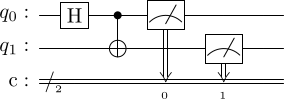
\includegraphics[width = .3 \linewidth]{images/circuit.png}
    \end{center}
    Before running the folded circuit, the circuit was ran with the above error, then again with measurement error mitigation. Resulting in the folowing histogram
    \begin{center}
        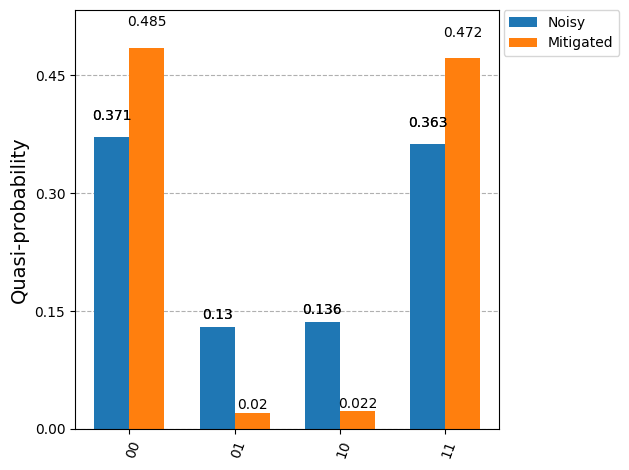
\includegraphics[width = .6 \linewidth]{images/hist1.png}
    \end{center}
    Then Zero-Noise Extrapolation (ZNE) was used with the scaling factors stated above.
    A linear fit was used to extract the raw expectation and zero-noise value.
    \begin{center}
        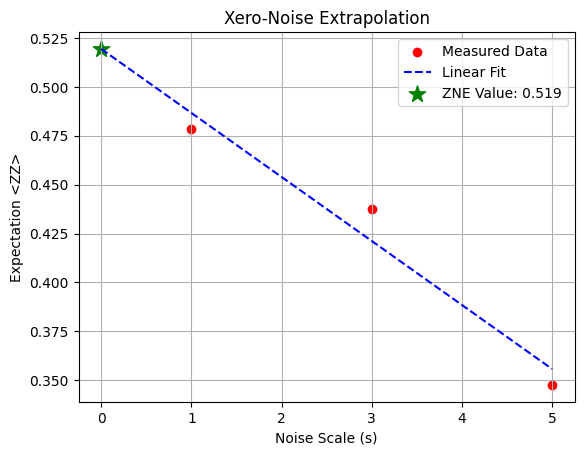
\includegraphics[width = .5 \linewidth]{images/linfit1.png}
    \end{center}
    \begin{align*}
        \text{Raw expectation: }&0.478515625\\
        \text{ZNE extrapolated: }&0.519368489583333
    \end{align*}
    \subsection{Questions}
    \begin{itemize}
        \item How close is the raw (unmitigated) value to the ideal value of 1?
        \begin{itemize}
            \item The raw expectation value is about 0.48, which is around half of what it should be.
        \end{itemize}
        \item Does ZNE move the result closer to the ideal value?
        \begin{itemize}
            \item Yes, for the given run, ZNE moved it closer by .04.
        \end{itemize}
        \item How large are the statistical fluctiations across runs?
        \begin{itemize}
            \item After running the code a few times (50 runs), I got raw expectation values between $0.37109375$ and $0.515625$ and extrapolated ZNE values between $0.3878580729166665$ and $0.5694986979166664$.
        \end{itemize}
    \end{itemize}
    \section{Increasing Fate Noise}
        The same setup was run again for new depolarizing values of $p = 0.1$ and $p = 0.2$.
        \subsection{$p = 0.1$}
            Using the same values as before, except for the depolarizing value, the circuit was again ran with error and error mitigation.
            \begin{center}
                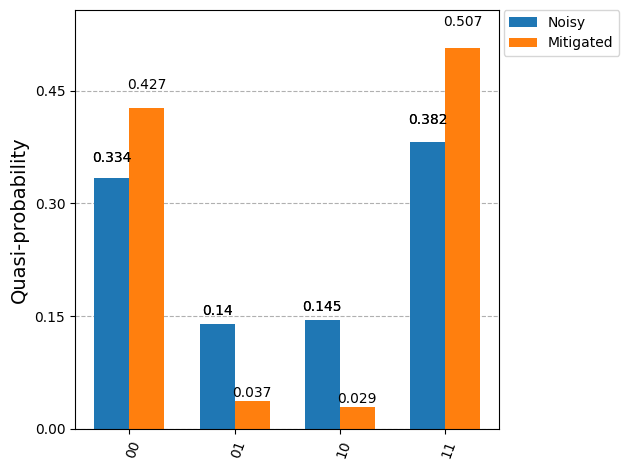
\includegraphics[width = .6 \linewidth]{images/hist2.png}
            \end{center}
            Then again with ZNE.
            \begin{center}
                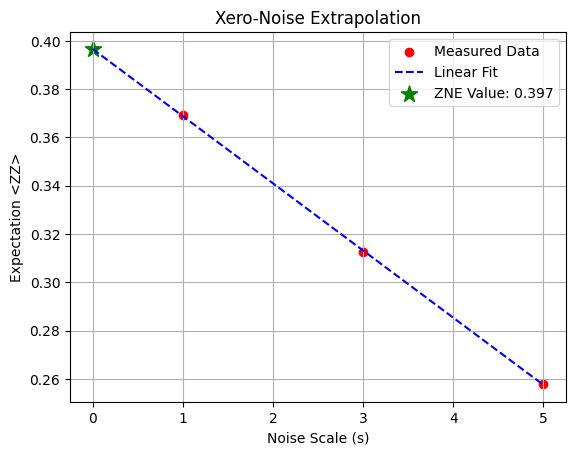
\includegraphics[width = .5 \linewidth]{images/linfit2.png}
            \end{center}
            \begin{align*}
                \text{Raw expectation: }&0.369140625\\
                \text{ZNE extrapolated: }&0.3966471354166664
            \end{align*}
        \subsection{$p = 0.2$}
            Using the same values as before, except for the depolarizing value, the circuit was again ran with error and error mitigation.
            \begin{center}
                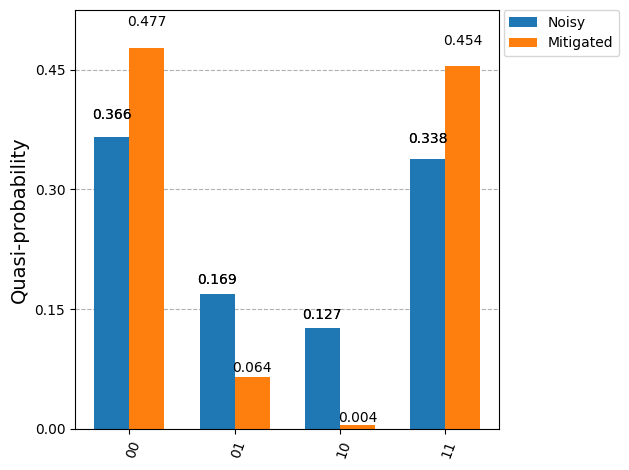
\includegraphics[width = .6 \linewidth]{images/hist3.png}
            \end{center}
            Then again with ZNE.
            \begin{center}
                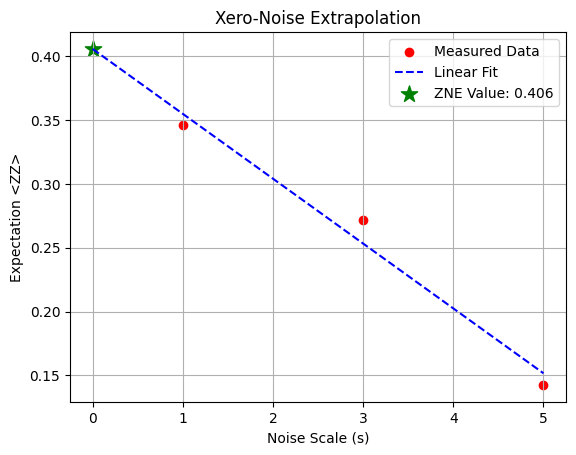
\includegraphics[width = .5 \linewidth]{images/linfit3.png}
            \end{center}
            \begin{align*}
                \text{Raw expectation: }&0.345703125\\
                \text{ZNE extrapolated: }&0.40559895833333304
            \end{align*}
    \subsection{Questions}
        \begin{itemize}
            \item At what noise level does ZNE stop improving the estimate?
            \begin{itemize}
                \item From testing noise values starting at 1 and working down I would say that the ZNE stops showing noticable imporvement around .07 error.
            \end{itemize}
            \item Does the linear extrapolation become unstable?
            \begin{itemize}
                \item Yes around this value (usually closer to 1) the linear extrapolation can give drastically diffent values due to the noise.
            \end{itemize}
            \item Do you observe extrapolated values outside the physical range $[-1,1]$?
            \begin{itemize}
                \item No, during my testing the values never left this bound even for higher, unstable values.
            \end{itemize}
        \end{itemize}
    \section{Increasing Folding Depth}
    The setup was replicated again, fixing $p$ at $0.05$, this time changing the set of scaling factors so $s \in \{1,3,5,7\}$. The histogram and linear fit are shown below.
    \begin{center}
        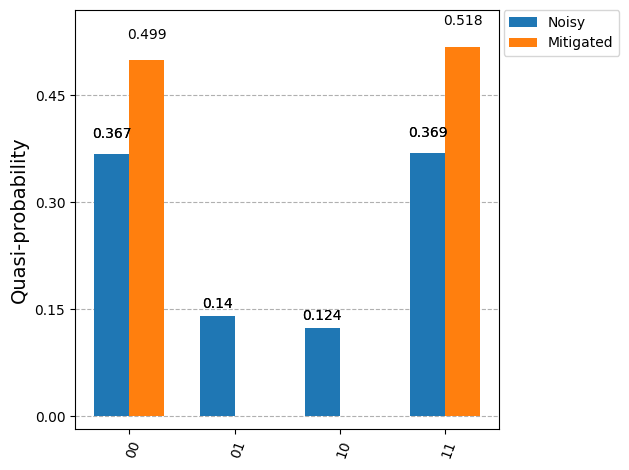
\includegraphics[width = .6 \linewidth]{images/hist4.png}
    \end{center}
    \begin{center}
        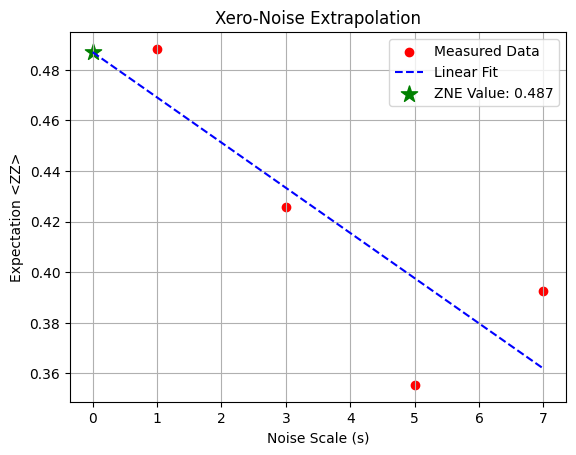
\includegraphics[width = .5 \linewidth]{images/linfit4.png}
    \end{center}
    \begin{align*}
        \text{Raw expectation: }&0.48828125\\
        \text{ZNE extrapolated: }&0.48701171875
    \end{align*}
    \subsection{Questions}
    \begin{itemize}
        \item Does adding more scale points improve or degrade the extrapolation?
        \begin{itemize}
            \item From this run, adding the extra scale point at 7, degrades the extrapolation and makes it worse then the raw value. For other runs the ZNE value is still better but by around 0.01 instead of 0.02 so still degrading.
        \end{itemize}
        \item How does the variance of the extrapolated value change?
        \begin{itemize}
            \item The variance is decreased and is more focused around .45 for both values.
        \end{itemize}
        \item Why does increased folding amplify statistical noise?
        \begin{itemize}
            \item We are introducing more gates, each with noise.
        \end{itemize}
    \end{itemize}
    \section{Reduced Shot Count}
    The setup from section 1 was replicated again, this time reducing the shots to 128. The histogram and linear fit are shown below.
    \begin{center}
        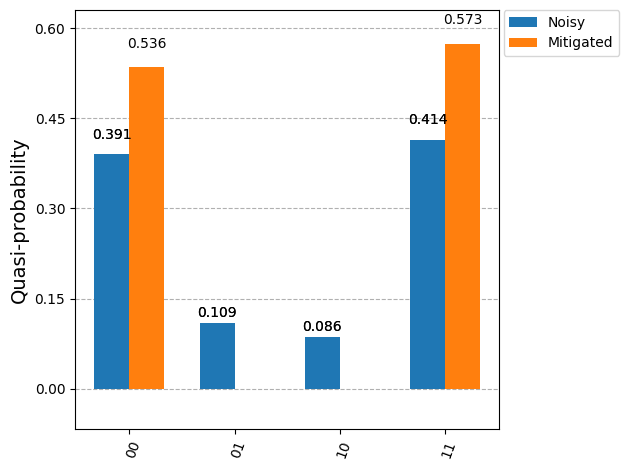
\includegraphics[width = .6 \linewidth]{images/hist5.png}
    \end{center}
    \begin{center}
        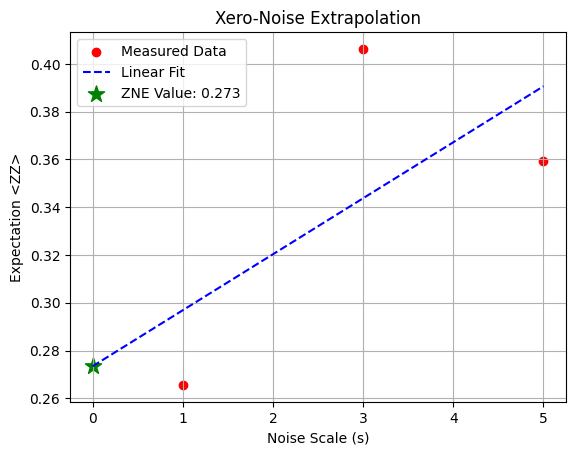
\includegraphics[width = .5 \linewidth]{images/linfit5.png}
    \end{center}
    \begin{align*}
        \text{Raw expectation: }&0.265625\\
        \text{ZNE extrapolated: }&0.27343749999999994
    \end{align*}
    \subsection{Questions}
    \begin{itemize}
        \item How sensitive is ZNE to shot noise?
        \begin{itemize}
            \item It appears that ZNE is fairly sensitive to shot noise as a decreased in shot noise does effect the effectiveness
        \end{itemize}
        \item Compare the raw and mitigated results under low statistics.
        \begin{itemize}
            \item Comparing the raw and mitigated results, they only differ by around .007. Both remain far off from the ideal value of 1.
        \end{itemize}
        \item Which source of uncertainty dominates?
        \begin{itemize}
            \item Due to the very small diffence, I would say the uncertainty is mostly statistical shot noise.
        \end{itemize}
    \section{Reflection}
        Error mitigation can reduce error but only for certain noise levels, folding depth and shot count. As the data shows, having a low shot count, high noise, or large folding depth can decreased the reliability of error mitigating techniques.
        Using error mitigation can correct part of inconsitensy, by compining multiple noisy measurements but this makes it more susceptible to statistical uncertainty.
    \end{itemize}

\end{document}